\chapter{\ifcpe ทฤษฎีที่เกี่ยวข้อง\else Background Knowledge and Theory\fi}

การทำโครงงานนี้เริ่มต้นจากการที่เราเล็งเห็นปัญหาของตารางสอบปลายภาคของมหาวิทยาลัยเชียงใหม่ 
ซึ่งตารางสอบของนักศึกษาบางคนอาจจะมีตารางเวลาที่ติดกันมากเกินไป ซึ่งผู้จัดทำเห็นว่าปัญหาการจัดตารางสอบปลายภาค
สามารถแปลงเป็นปัญหาที่มีวิธีในการแก้ไขอยู่แล้วได้ ในบทนี้จะกล่าวถึงผลการศึกษาค้นคว้าทฤษฎีที่เกี่ยวข้อง งานวิจัย หรือโครงงาน ที่เคยมีผู้นำเสนอไว้แล้ว
เพื่อช่วยอธิบายถึงสิ่งต่าง ๆ ที่เกี่ยวข้องกับโครงงานนี้เพื่อให้ผู้อ่านเข้าใจเนื้อหาในบทถัด ๆ ไปได้ง่ายยิ่งขึ้น โดยในบทนี้จะมีเนื้อหาต่าง ๆ ได้แก่ literature review 
และงานเขียนอื่น ๆ ที่เกี่ยวข้องกับการสร้างระบบจัดตารางสอบ
ซึ่งจะกล่าวถึงงานวิจัยต่าง ๆ ที่ได้ศึกษามา และส่วนของอัลกอริทึมที่เกี่ยวข้อง ซึ่งจะกล่าวถึงรูปแบบและวิธีการทำงานของอัลกอริทึมต่าง~ๆ 

\section{Literature review and related work}
การกำหนดเวลาสอบปลายภาคเพื่อหลีกเลี่ยงปัญหาที่นักศึกษาคนใด ๆ มีวิชาที่ต้องสอบมากกว่าหนึ่งวิชาในช่วงเวลาเดียวกันสามารถแก้ไขได้ด้วยวิธีการต่าง ๆ มากมาย
เช่น วิธีการ metaheuristic ซึ่งสามารถหาวิธีการแก้ปัญหาที่ดี ได้ในระยะเวลาที่เหมาะสม~\cite{meta-for-vertexcolor}
และสามารถกำหนดข้อจำกัดหรือเงื่อนไขต่าง ๆ ให้กับตารางสอบได้ ซึ่งทำให้สามารถกำหนดขอบเขตของผลลัพธ์ได้ แต่อาจจะไม่ได้วิธีแก้ปัญหาที่ดีที่สุด

อีกวิธีการที่สามารถใช้แก้ไขปัญหาการจัดตารางสอบได้ก็คือการใช้ memetic algorithms (MA) ซึ่งเป็นวิธีการที่นำ local search มาประยุกต์ใช้กับ genetic algorithm 
เพื่อช่วยให้คำตอบของปัญหานั้น converge ช้าลง \cite{pablo-memetic-algo} ซึ่ง Ender {\"O}zcan เคยได้นำวิธีการนี้มาประยุกต์ใช้ในการแก้ปัญหาการจัดตารางสอบ 
โดยได้สร้าง framework สำหรับออกแบบตัวดำเนินการที่ใช้ในการ crossover และ mutation ของ genetic algorithm ด้วย~\cite{fes}
โดยในการทดลองนี้ได้มีการคำนึงถึงนักศึกษา โดยกำหนดข้อจำกัดของตารางสอบที่ได้ให้ไม่มีนักศึกษาที่ต้องสอบติดกันสองวิชาในแต่ละวัน แต่การจัดตารางสอบในแบบของ {\"O}zcan 
นั้นเป็นการจัดตารางสอบของมหาวิทยาลัย Yeditepe โดยแบ่งตารางสอบเป็นของภาควิชาต่าง ๆ และแบ่งย่อยแยกตามสาขาวิชาอีกที วิธีการนี้ไม่สามารถนำมาใช้กับการจัดตารางสอบของมหาวิทยาลัยเชียงใหม่ได้
เนื่องจากมหาวิทยาลัยเชียงใหม่ มีวิชาศึกษาทั่วไปซึ่งเป็นวิชาที่เปิดให้นักศึกษาจากต่างคณะสามารถลงทะเบียนได้ทำให้มีนักศึกษาเป็นจำนวนมากกว่าที่ความจุที่นั่งสอบของคณะนั้นจะรับไหว
ซึ่งทำให้การจัดตารางสอบโดยใช้วิธีนี้นั้นเป็นไปได้ยากเพราะจำนวนนักศึกษาที่เกินความจุที่นั่งสอบนั้นจะละเมิดข้อจำกัดที่กำหนดไว้ 

นอกจากวิธีที่กล่าวมาข้างต้น ปัญหาการกำหนดเวลาสอบ นั้นเป็นปัญหาประเภท scheduling problem 
ซึ่งเป็นปัญหาที่สามารถแปลงส่วนประกอบของปัญหาให้อยู่ในรูปของปัญหา graph coloring~\cite{mcs} ได้ 
โดยจะได้กราฟ ที่มีจุดเป็นรายวิชาพร้อมจำนวนนักศึกษาลงทะเบียน และมีเส้นเชื่อมคู่วิชาที่มีนักศึกษาลงทะเบียนทั้งคู่
โดยมีน้ำหนักเส้นเป็นจำนวนนักศึกษาดังกล่าว โดยจุดสองจุดใด ๆ ในกราฟที่มีเส้นเชื่อมกันจะถูกกำหนดสีให้ต่างกัน
ซึ่งแสดงถึงวันและเวลาที่จัดสอบปลายภาคในวิชานั้น ๆ โดยจุดที่มีคนละสีก็จะถูกจัดให้สอบคนละช่วงเวลากัน

การแปลงปัญหาการจัดตารางสอบปลายภาคให้เป็นปัญหา graph coloring ถึงแม้จะไม่กำหนดข้อจำกัดใด ๆ เพิ่มเติมเลย
ปัญหา graph coloring ก็เป็นปัญหา NP-complete ด้วยตัวเองอยู่แล้ว~\cite{alg-design} 
ซึ่งหมายความว่ายังไม่สามารถหาอัลกอริทึมที่ใช้เวลา polynomial-time ในการแก้ไขปัญหาให้ได้ผลลัพธ์ที่เหมาะสมที่สุด
ดังนั้นการใช้วิธี graph coloring เพื่อแก้ปัญหานี้อาจจะใช้เวลานานในการหาตารางสอบ หากจำนวนของโหนดของกราฟมีจำนวนมาก ๆ
แต่หากคำนึงถึงวิชาต่าง ๆ ที่เปิดสอนภายในมหาวิทยาลัยแล้ว จำนวนโหนดซึ่งก็เท่ากับจำนวนวิชาที่เปิดสอนนั้นมีไม่มากขนาดที่จะทำให้อัลกอริทึมที่ใช้หาผลลัพธ์นั้นช้าจนเกินไป

ในงานของ Mohammad Malkawi และคณะ~\cite{graphcl-2008}
ได้มีการทดลองใช้ graph coloring algorithm ในการจัดตารางสอบของมหาวิทยาลัย โดยมีการคำนึงถึงความเป็นธรรม (fairness) ความถูกต้องของตารางสอบ (accuracy) และ ความเหมาะสมของจำนวนวันที่สอบ (optimal exam time period)
โดยได้มีการกำหนดข้อจำกัดต่าง ๆ ที่เปลี่ยนแปลงได้ตามต้องการ เช่น จำนวนช่วงเวลาที่จัดสอบได้ในหนึ่งวัน จำนวนวิชาที่จัดสอบพร้อมกันได้ในหนึ่งวัน จำนวนวิชาที่นักศึกษาหนึ่งคนสามารถสอบได้มากที่สุดในหนึ่งวัน
จำนวนวันเว้นว่างที่นักศึกษาหนึ่งคนจะมีได้ระหว่างการสอบวิชาถัดไป โดยในงานวิจัยนี้อัลกอริทึมจะจัดตารางสอบโดยให้ได้จำนวนวันสอบที่น้อยที่สุด (minimize the number of exam
slots and/or number of exam days) ซึ่งจากผลการทดลองนั้นข้อมูลที่ต้องประมวลผล มีจำนวนวิชาที่ต้องจัดสอบทั้งหมด 1092 วิชา โดยกราฟที่สร้างขึ้นมามีดีกรีเฉลี่ยที่ 54 และมีโหนดที่มีดีกรีมากที่สุดมีดีกรีเท่ากับ 434
โดยเวลาที่อัลกอริทึมใช้ในการจัดตารางสอบนั้นเฉลี่ยอยู่ที่ 90 วินาทีต่อรอบ แต่ในงานนี้นั้นมีข้อจำกัดบางอย่างที่ไม่ได้คำนึงถึง เช่น จำนวนที่นั่งสอบของมหาวิทยาลัย การที่นักศึกษามีสอบติดกันหลายวิชา และการให้ความสำคัญกับช่วงเวลาในการสอบ

ในงานของ E. Burke และคณะ~\cite{graphcl-constr-manip} และงานของ Timothy Redl~\cite{graphcl-alter-approach}
ได้มีการใช้ graph coloring algorithm ในการจัดตารางสอบให้กับมหาวิทยาลัยเหมือนกันและมีการจัดห้องสอบให้กับวิชาต่าง ๆ ด้วย
แต่งานทั้งสองแตกต่างกันที่ตรงที่งานของ E. Burke~\cite{graphcl-constr-manip} แยกอัลกอริทึมในการจัดตารางสอบกับอัลกอริทึมในการจัดห้องสอบออกจากกัน
และทำงานแยกกัน โดยมี hard constraint คือในแต่ละวิชาที่จัดสอบต้องสอบภายในห้องเดียวกัน แต่งานของ Timothy Redl~\cite{graphcl-alter-approach}
นั้นการจัดห้องสอบจะถูกจัดให้กับแต่ละวิชาในขณะเดียวกันกับขั้นตอนการระบายสีกราฟเลย

ในงานของ Barry McCollum และคณะ~\cite{auto-timetable} 
ไม่ได้นำเสนอถึงอัลกอรึทึมในการจัดตารางสอบโดยตรง แต่ได้นำเสนอ model สำหรับแก้ปัญหาการจัดตารางสอบที่นักวิจัยได้พยายามแก้ปัญหานี้กันมาอย่างยาวนาน
โดยได้แสดงให้เห็นถึงความพยายามที่จะหาอัลกอริทึมในการจัดตารางสอบหลากหลายรูปแบบพร้อมคำอธิบายคร่าว ๆ และได้มีการนิยามปัญหาการจัดตารางสอบรูปแบบต่าง ๆ
และนิยามข้อจำกัดที่ใช้เป็นเกณฑ์ทำหรับการประเมินตารางสอบที่ได้จากระบบ ทั้ง required, hard, และ soft constraints พร้อมคำอธิบายอย่างละเอียดและครบถ้วน 
และได้มีการยกตัวอย่าง constraints ในรูปแบบต่าง ๆ ที่เป็นข้อจำกัดที่เราคำนึงถึงในการจัดตารางสอบในทางปฏิบัติ เช่น การจัดห้องสอบหนึ่งวิชาต้องไม่แยกสอบหลายห้อง 
การจัดเวลาสอบให้วิชาที่มีหลายตอนต้องจัดในเวลาเดียวกัน การจัดสอบวิชาที่มีนักศึกษาลงทะเบียนเยอะควรจัดสอบก่อนเพื่อให้อาจารย์ผู้สอนได้มีเวลาตรวจข้อสอบมากขึ้น และยังได้มีการพูดถึงข้อจำกัดที่คำนึงถึงนักศึกษาที่สอบด้วย เช่น การที่นักศึกษาคนใด ๆ มีสอบสองวิชาติดกัน หรือ มีสอบหลายวิชาในวันเดียวกัน 
รวมถึงวันเว้นว่างระหว่างการสอบสองวิชาของนักศึกษาคนใด ๆ ด้วย โดยในงานนี้ได้มีการนิยาม model การแก้ปัญหานี้ด้วย integer programming (IP)

ในงานของ Sandeep Saharan และ Ravinder Kumar~\cite{graphcl-idepset}
ได้มีการใช้ graph coloring algorithm ร่วมกับการใช้ independent set
เพื่อจัดตารางสอบพร้อมทั้งจัดห้องสอบให้กับแต่ละวิชาด้วย โดยมีตัวแปรและข้อกำหนดที่คำนึงถึงได้แก่ จำนวนที่นั่งสอบ และกรรมการคุมสอบ
เป้าหมายหลักของงานนี้คือ การใช้ทรัพยากรต่าง ๆ ทั้งที่นั่งสอบและกรรมการคุมสอบให้เกิดประโยชน์สูงสุด (optimize resource utilization)
โดยในงานได้ใช้ graph coloring algorithm ในการจัดช่วงเวลาสอบให้กับแต่ละวิชาก่อน โดยจัดให้ใช้ช่วงเวลาที่สอบน้อยที่สุด
จากนั้นจึงจัดห้องสอบให้กับแต่ละวิชาโดยมีข้อจำกัดคือแต่ละวิชาที่สอบห้ามแยกห้องสอบ โดยจัดห้องสอบให้กับวิชาที่มีนักศึกษาลงทะเบียนมากกว่าก่อน
หลังจากจัดห้องสอบได้แล้วจะมีวิชาที่ไม่สามารถจัดห้องสอบได้เพราะที่นั่งไม่เพียงพอ 
จะนำข้อจำกัดที่ว่าแต่ละวิชาที่สอบห้ามแยกห้องสอบออก และจัดห้องสอบให้กับวิชาที่เหลือ
โดยในงานนี้ได้คำนึงถึงการจัดการกับที่นั่งสอบและกรรมการคุมสอบเป็นหลัก แต่ไม่ได้มีการคำนึงถึงข้อจำกัดเกี่ยวกับวิชาต่าง ๆ และข้อจำกัดเกี่ยวกับความเหมาะสมของเวลาสอบของนักศึกษา

\iffalse
\section{Tools}
\subsection{Gurobi Optimizer}
Gurobi Optimizer เป็น Solver ที่ใช้สำหรับแก้ปัญหา optimization โดยที่จะเน้นไปทางด้านของปัญหาต่าง ๆ ดังนี้ 
\begin{itemize}
  \item Linear programming (LP)
  \item Mixed-integer linear programming (MILP)
  \item Quadratic programming (QP)
  \item Mixed-integer quadratic programming (MIQP)
  \item Quadratically-constrained programming (QCP)
  \item Mixed-integer quadratically-constrained programming (MIQCP)
\end{itemize}
ผลลัพธ์ที่ได้จาก Gurobi Optimizer อาจนำมาใช้เป็นตัวเปรียบเทียบประสิทธิภาพกับผลลัพธ์การทำงานที่ได้จากอัลกอริทึมของเรา
\fi

\section{หลักการ แนวคิด และทฤษฏีที่เกี่ยวข้องในการทำโครงงาน }
\subsection{Metaheuristics}
Meta­heuristics~\cite{metaheuris} เป็นวิธีหนึ่งในการแก้ไขปัญหา optimization problems ซึ่งเป็นที่นิยม เนื่องจากใช้งานได้ดีและเหมาะสมกับเวลาที่ใช้ในการประมวลผล
โดยวิธีเหล่านี้นั้นส่วนใหญ่จะเป็นวิธีการที่มีแรงบันดาลใจมาจากการเลียนแบบหลักการของธรรมชาติและนำมาดัดแปลงเป็นอัลกอริทึมเพื่อใช้ในการแก้ปัญหาต่าง ๆ ตัวอย่างของ metaheuristic algorithms เช่น genetic algorithm, evolutionary computation, simulated annealing, tabu search เป็นต้น
\subsection{Genetic algorithms}
Genetic algorithms เป็นเทคนิคหนึ่งใน metaheuristics สำหรับค้นหาผลลัพธ์หรือคำตอบโดยประมาณของปัญหา โดยอาศัยหลักการจากทฤษฎีวิวัฒนาการทางชีววิทยาและหลักการคัดเลือกตามธรรมชาติ  กล่าวคือ สิ่งมีชีวิตที่เหมาะสมที่สุดจึงจะอยู่รอด \cite{ga} โดยกระบวนการคัดเลือกได้เปลี่ยนแปลงสิ่งมีชีวิตให้เหมาะสมยิ่งขึ้นด้วยตัวดำเนินการทางพันธุกรรม เช่น การสืบพันธุ์ การแลกเปลี่ยนยีน การกลายพันธุ์ เป็นต้น โดยขั้นตอนการทำงานของ genetic algorithms มีดังนี้ 
\begin{enumerate}
  \item initial population เป็นขั้นตอนเริ่มต้นของอัลกอริทึมซึ่งจะทำการกำหนดชุดข้อมูลผลลัพธ์ เรียกชุดข้อมูลนี้ว่า population ซึ่งชุดข้อมูลนี้จะประกอบไปด้วยผลลัพธ์ที่ถูกเข้ารหัสในรูปแบบของสายอักขระที่แต่ละอักขระเป็นบิต 0 หรือ 1 เรียกแต่ละบิตนี้ว่า gene
  โดยที่แต่ละสายอักขระที่ประกอบจาก genes นี้เรียกว่า chromosome โดยชุดข้อมูลนี้อาจจะสุ่มแต่ละ gene ขึ้นมาเป็นค่าเริ่มต้น
  \item fitness function เป็น function สำหรับใช้ในการคัดเลือกชุดข้อมูลที่เหมาะสมให้สามารถอยู่ต่อไปได้ โดยจะมีการคำนวณค่า fitness scores ให้กับแต่ละ chromosome
  โดย fitness scores จะขึ้นอยู่กับความพอใจในผลลัพธ์ที่ได้ของผู้พัฒนา
  \item genetic operator คือวิธีการในการปรับเปลี่ยนรูปแบบโครงสร้างของ chromosome ที่เหมาะสมสำหรับรุ่นถัดไปของกระบวนการ ซึ่งมีวิธีการอยู่ 3 แบบหลัก ๆ ได้แก่
  \begin{itemize}
  \item selection เป็นการเลือกคู่ chromosome ของข้อมูลที่เหมาะสม เพื่อให้ chromosome คู่นี้ส่งต่อ gene ที่ดีแล้วไปยัง chromosome รุ่นถัดไป โดยจะเลือก chromosome ที่มีค่า fitness scores มากที่สุด
  \item crossover เป็นการสุ่มเลือกตำแหน่งระหว่าง genes จาก parent chromosome 1 คู่ โดย genes ด้านซ้ายหรือขวาของจุดแบ่งจะถูกสับเปลี่ยนกันระหว่าง parent chromosome คู่นั้น
  \item mutation เป็นการสุ่มกลับค่าของ gene ใน chromosome ให้มีค่าตรงกันข้ามโดยมีค่าความน่าจะเป็นที่จะเกิด mutation ต่ำ ๆ เพื่อป้องกันไม่ให้ผลลัพธ์ converge ก่อนที่ควรจะเป็น
\end{itemize}
\end{enumerate}
Genetic algorithms สามารถจบการทำงานได้หลายวิธี โดยมีเงื่อนไขในการจบการทำงานดังนี้
\begin{itemize}
  \item เมื่อ population เปลี่ยนผ่านไปถึงรุ่นที่ต้องการแล้ว 
  \item เมื่อ population ไม่มีการพัฒนาแล้ว หรือไม่มีการเปลี่ยนแปลงไปในทางที่ดีขึ้นเป็นระยะเวลาหนึ่ง
  \item เมื่อ fitness scores ของ population มีค่าเท่าที่ต้องการแล้ว
\end{itemize}

\subsection{Graph coloring}
 
Graph coloring เป็นปัญหาที่ได้รับความสนใจอย่างยิ่งในเรื่องทฤษฎีกราฟซึ่งเป็นปัญหาที่เกี่ยวกับการพยายามระบายสีจุดของกราฟ โดยให้จุดที่อยู่ติดกันมีสีต่างกันและใช้สีให้น้อยที่สุด
การระบายสีกราฟอาจมีหลายรูปแบบ บางรูปสามารถใช้สีเพียงสองสีก็เพียงพอที่จะให้จุดที่อยู่ติดกันมีสีต่างกัน บางรูปจำเป็นต้องใช้หลายสีถึงจะเพียงพอที่จะให้จุดที่อยู่ติดกันมีสีต่างกัน 
ดังนั้นจะเรียกจำนวนสีอย่างน้อยที่สุดที่เพียงพอที่จะให้จุดที่อยู่ติดกันมีสีต่างกันว่า จำนวนสีของกราฟ (chromatic number) ซึ่งวิธีการระบายสีกราฟมักจะถูกนำไปประยุกต์ใช้กับการแก้ปัญหาการกำหนดตารางเวลา (scheduling problem) 

\subsection{Breadth-first search}
Breadth-first search หรือการค้นหาตามแนวกว้าง เป็นขั้นตอนวิธีในการท่องกราฟอย่างหนึ่ง โดยในขณะที่กำลังท่องกราฟมายังจุดยอดหนึ่ง ๆ นั้น จะมีการกระทำสองอย่างคือ: (ก) เข้าเยี่ยมและตรวจสอบจุดยอดดังกล่าว (ข) เข้าถึงจุดยอดข้างเคียงของจุดยอดดังกล่าว
โดยเริ่มที่จุดยอดเริ่มต้นของกราฟ (root) และทำการสำรวจจุดยอดที่ติดกัน (adjacent node) ไปทีละจุดยอด
โดยสำรวจลงไปทีละระดับของโครงสร้างกราฟ โดยเริ่มจากระดับแรกที่ root แล้วลงมาระดับที่ 1 จากซ้ายไปขวา เมื่อเสร็จระดับที่ 1 จะค่อยไปสำรวจที่ระดับที่ 2 จากซ้ายไปขวาเช่นกัน ทําเช่นนี้เรื่อย ๆ 
จนครบทุกจุดยอด โดยมีตัวอย่างลําดับการเดินทางด้วยการค้นหาตามแนวกว้างเป็นไปตามหมายเลขที่กํากับไว้บนจุดยอด ดังรูปที่ \ref{fig:graph_bfs}
\begin{figure}
  \begin{center}
    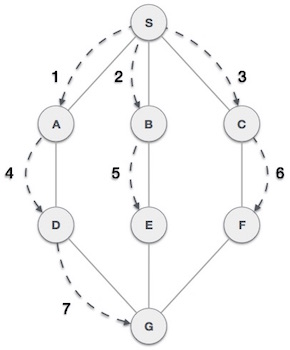
\includegraphics[width=0.5\textwidth]{images/breadth_first_traversal.jpg}
  \end{center}
  \caption[ตัวอย่างการทำ BFS บนกราฟ]{ตัวอย่างการทำ BFS บนกราฟ}
  \label{fig:graph_bfs}     
\end{figure}
\section{\ifcpe%
ความรู้ตามหลักสูตรซึ่งถูกนำมาใช้หรือบูรณาการในโครงงาน
\else%
ISNE knowledge used, applied, or integrated in this project
\fi
}
\begin{itemize}
  \item 261218 Algorithms for Computer Engineers ได้นำวิธีดำเนินงาน หลักการและทฤษฏี ดังนี้มาใช้เพื่อแก้ไขปัญหาในโครงงานนี้  
  \begin{itemize}
  \item วิธีการคิดและวิเคราะห์ปัญหา
  \item วิธีการแปลงปัญหาใหญ่ที่แก้ไขยากให้กลายเป็นปัญหาย่อยที่เล็กกว่าเพื่อใช้วิธีการที่มีอยู่แล้วในการแก้ไขปัญหาย่อยนั้นและนำไปสู่การแก้ปัญหาใหญ่ได้สำเร็จ
  \item ทฤษฏี graph coloring
  \item การแก้ปัญหา scheduling problem
  \item การแก้ปัญหา NP-complete และ NP-hard
  \end{itemize}
\end{itemize}

\section{\ifcpe%
ความรู้นอกหลักสูตรซึ่งถูกนำมาใช้หรือบูรณาการในโครงงาน
\else%
Extracurricular knowledge used, applied, or integrated in this project
\fi
}
ความรู้นอกหลักสูตรที่ใช้สำหรับการแก้ไขปัญหาของโครงงานเพื่อให้ได้ผลลัพธ์ที่เหมาะสุดที่สุด เราได้ทำการศึกษา หลักการและทฤษฏี ดังนี้
\begin{itemize}
  \item Meta­heuristics
  \item Genetic algorithms
  \item การสร้างเว็บแอพพลิเคชันด้วย Vue.js, Node.js, Express
  \item การใช้งานฐานข้อมูล MongoDB
\end{itemize}
